\documentclass[11pt]{article}

\usepackage{times} % Times New Roman font
\usepackage{graphicx} % For images
\usepackage{enumitem} % For numbered items
\usepackage{lipsum} % For dummy text
\usepackage{hyperref} % For references
\hypersetup{
    colorlinks=true,
    linkcolor=blue,
    filecolor=magenta,      
    urlcolor=cyan,
} % For hyperlinks
\usepackage{amsmath} % For math equations
\usepackage{cleveref} % For clever references
\crefname{appendix}{Appendix}{Appendices}
\usepackage{fancyvrb} % For code display
\usepackage{fancyhdr} % For custom headers
\usepackage{pythonhighlight} % For Python code
\usepackage{float} % For image positioning
\usepackage{amsmath} % For math equations
\usepackage{xcolor} % For custom colors
\usepackage{natbib} % For bibliography
\usepackage{appendix} % For appendices
\usepackage[font={small,it}]{caption} 
% \usepackage{mwe}% For custom captions
\usepackage{listings}
\usepackage{color}
\usepackage{amsmath}
\usepackage{graphicx}
\usepackage{hyperref}
\usepackage{geometry}
\usepackage{caption}
\captionsetup{font={small, sf}}
\usepackage{ctex}
\usepackage{siunitx}
\usepackage{booktabs}
\renewcommand{\tablename}{Table}
\renewcommand{\figurename}{Figure}
\renewcommand{\abstractname}{Abstract}
\geometry{a4paper, margin=1in}
\definecolor{codegreen}{rgb}{0,0.6,0}
\definecolor{codegray}{rgb}{0.5,0.5,0.5}
\definecolor{codepurple}{rgb}{0.58,0,0.82}
\definecolor{backcolour}{rgb}{0.95,0.95,0.92}
\usepackage{fancyhdr}
\setlength{\headheight}{13.59999pt}
\addtolength{\topmargin}{-1.59999pt}

\lstdefinestyle{mystyle}{
    backgroundcolor=\color{backcolour},
    commentstyle=\color{codegreen},
    keywordstyle=\color{magenta},
    numberstyle=\tiny\color{codegray},
    stringstyle=\color{codepurple},
    basicstyle=\ttfamily\footnotesize,
    breakatwhitespace=false,
    breaklines=true,
    captionpos=b,
    keepspaces=true,
    numbers=left,
    numbersep=5pt,
    showspaces=false,
    showstringspaces=false,
    showtabs=false,
    tabsize=2
}

\lstset{style=mystyle}

\lstnewenvironment{outputlisting}{
  \lstset{
    basicstyle=\ttfamily\footnotesize,
    frame=single,
    backgroundcolor=\color{lightgray},
    keywordstyle=\color{blue},
    breaklines=true,
    postbreak=\mbox{\textcolor{red}{$\hookrightarrow$}\space},
    xleftmargin=.1\textwidth,
    xrightmargin=.1\textwidth,
    captionpos=b,
    language=[Sharp]C,
    numbers=none,
    tabsize=2,
    showstringspaces=false
  }
}{}

\title{Complex Network Analysis of Classical Chinese Literature: Insights from the Confucian Canon of Scripta Sinica Corpus}
\author{Yichi Zhang u7748799}
\date{May, 2024}

\begin{document}

\maketitle

\thispagestyle{fancy}

\begin{abstract}
    The study of language 
\end{abstract}

\section{Introduction}

\section{Data and Methods}

\subsection{Scripta Sinica Corpus}

\subsection{Network Construction}

\subsubsection{Character Co-occurrence Network (CCN)}

\subsubsection{Character-Sentence Network (CSN)}

\subsection{Network Analysis Methods}

\section{Models and Results}
This section presents the main findings of our study on the topological properties of CCN and CSN. We focus on the small-world properties, scale-free characteristics, disassortativity and hierarchical structure. These results provide valuable insights into the organizational principles and structural features of Chinese language networks.
\subsection{Small-World Properties}

Compared to a random network with same scale, if a specific network maintains a similar average shortest path length and has a larger clustering coefficient, it is considered to have small world properties \cite{Watts1998}. Therefore, we investigated the clustering coefficient, and average shortest path length of CCN and CSN to assess their small world properties.
\begin{figure}[htbp]
    \centering
    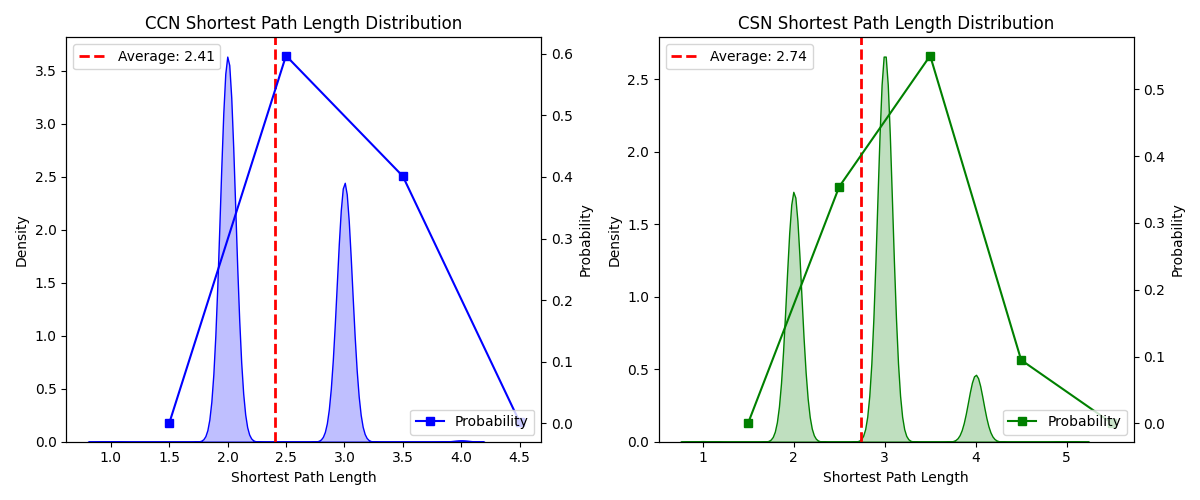
\includegraphics[width=0.8\textwidth]{../analysis/shortest path/shortest path.png}
    \caption{Shortest path length distributions of CCN and CSN. The average shortest path lengths are 2.41 for CCN and 2.74 for CSN.}
    \label{fig:shortest_path}
    \end{figure}
    Compared to an equivalent random network ($C_{\rm rand}=2.83 \times 10^{-5}, L_{\rm rand}=3.66$), CCN has a significantly higher clustering coefficient $C_1=0.022$ and a slightly lower average shortest path length $L_1=2.41$. Similarly, CSN has a higher $C_2=0.046$ and a lower $L_2=2.74$ ($C_{\rm rand}=1.20 \times 10^{-4}, L_{\rm rand}=2.93$). These findings suggest that Classical Chinese lexical networks have strong small-world effects, making information processing and retrieval easier due to their highly connected local clusters and efficient global communication.
\subsection{Scale-Free Characteristics and Matthew Effect}
Many real-world networks exhibit a power-law degree distribution, indicating a scale-free structure \cite{Barabasi1999}:
\begin{equation}
P(k) \sim k^{-\gamma}
\end{equation}
\begin{figure}[htbp]
    \centering
    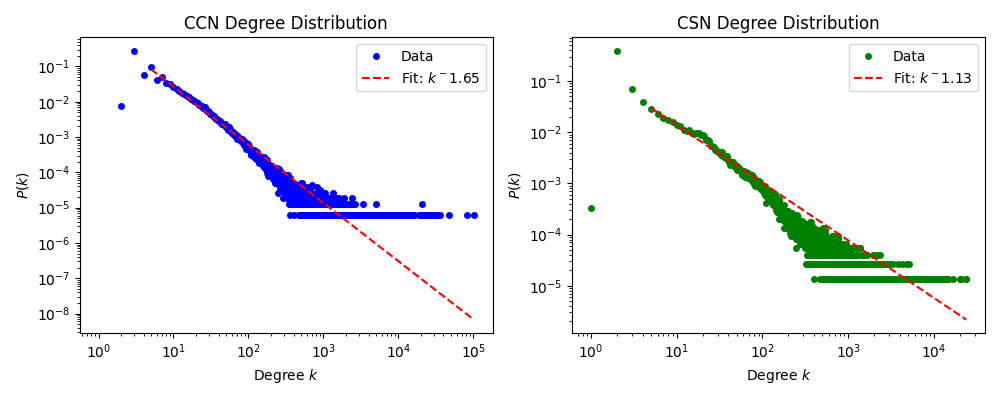
\includegraphics[width=0.8\textwidth]{../analysis/degree distribution/degree distribution.png}
    \caption{Degree distributions of CCN and CSN on a double logarithmic scale. The power-law exponents are 1.65 for CCN and 1.13 for CSN.}
    \label{fig:degree_dist}
    \end{figure}
    The degree distribution $P(k)$ represents the probability that a randomly selected node in the network has degree $k$. Figure \ref{fig:degree_dist} shows the degree distributions of CCN and CSN on a double logarithmic scale. Both networks exhibit power-law tails, indicating a scale-free structure.
    The scale-free nature suggests that a small number of highly connected characters (e.g., function words and common content words, which are usually single characters rather than word combinations in Classical Chinese) play a crucial role in maintaining the connectivity of the Classical Chinese language system.
    To further investigate the relationship between node importance and connection strength, we analyzed the node strength distribution and its correlation with degree.
\begin{figure}[htbp]
    \centering
    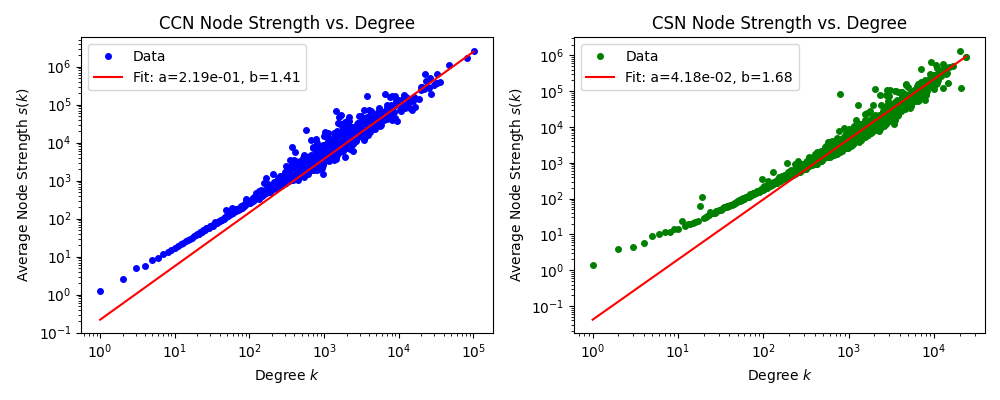
\includegraphics[width=0.8\textwidth]{../analysis/node strength/node strenth.png}
    \caption{Average node strength $s(k)$ vs. degree $k$ for the CCN and CSN networks on a double logarithmic scale. The data is fitted to a power law $s(k) = ak^b$. For CCN, $a=2.19e-01$ and $b=1.41$, indicating a super-linear scaling of node strength with degree. For CSN, $a=4.18e-02$ and $b=1.68$, also showing a super-linear scaling but with a higher exponent compared to CCN.}
    \label{fig:strength_dist}
    \end{figure}
    Figure \ref{fig:strength_dist} shows the node strength distributions of CCN and CSN on a double logarithmic scale. Both networks exhibit heavy-tailed distributions, indicating a highly heterogeneous allocation of connection strengths among nodes. 
    Moreover, we observed a super-linear relationship between node strength $s(k)$ and degree $k$ (Figure \ref{fig:strength_dist}):
    \begin{equation}
    s(k) \sim k^{\alpha}
    \end{equation}
    For CCN, the fitted exponent is $\alpha=1.41$, while for CSN, $\alpha=1.68$. This result suggests that high-degree nodes tend to have disproportionately larger strengths compared to low-degree nodes, reflecting the preferential attachment mechanism commonly observed in evolving networks and pointing to a "Matthew effect" or "rich-get-richer" phenomenon \cite{Barabasi1999}.
\subsection{Hierarchical Structure and Disassortativity}
By observing the power-law relationship between the clustering coefficient $C(k)$ and the node degree $k$ \cite{Ravasz2003}, we can examine whether a complex network possesses a hierarchical structure:
\begin{equation}
C(k) \sim k^{-\beta}
\end{equation}
\begin{figure}[htbp]
    \centering
    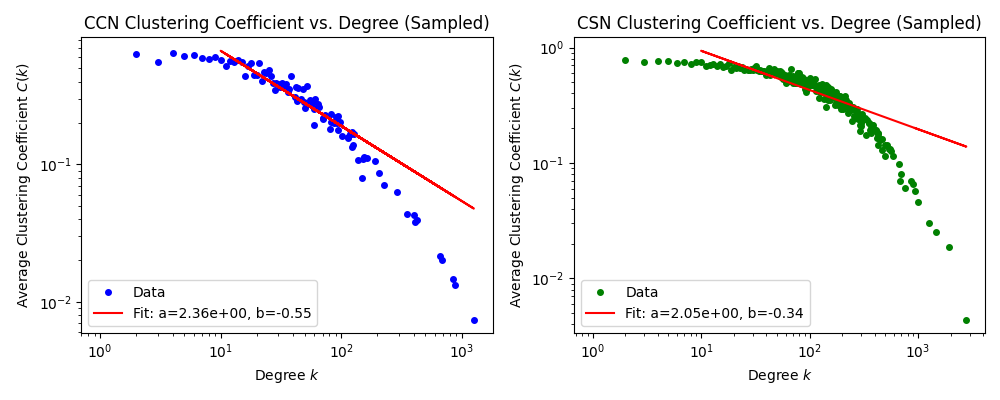
\includegraphics[width=0.8\textwidth]{../analysis/clustering coefficient/clustering coefficient.png}
    \caption{Average clustering coefficient $C(k)$ vs. degree $k$ for the CCN and CSN networks on a double logarithmic scale, using sampled data. The data is fitted to a power law $C(k) = ak^b$. For CCN, $a=2.36e+00$ and $b=-0.55$, indicating a sub-linear decrease of clustering coefficient with degree. For CSN, $a=2.05e+00$ and $b=-0.34$, also showing a sub-linear decrease but with a slower decay compared to CCN.}
    \label{fig:hierarchical}
    \end{figure}
    The hierarchical structures of CCN and CSN reflect the multi-scale, modular organization of the Chinese language system, as shown in Figure \ref{fig:hierarchical}, with $\beta=0.55$ for CCN and $\beta=0.34$ for CSN. There are tightly connected groups at various linguistic unit levels, from radicals to words and phrases.
    In addition, we studied the degree correlations in CSN and CCN to understand the assortativity of the networks. Disassortative mixing is the tendency of high-degree nodes to connect with low-degree nodes, measured by a negative degree correlation coefficient $r$ \cite{Newman2002}.
    
\begin{figure}[htbp]
    \centering
    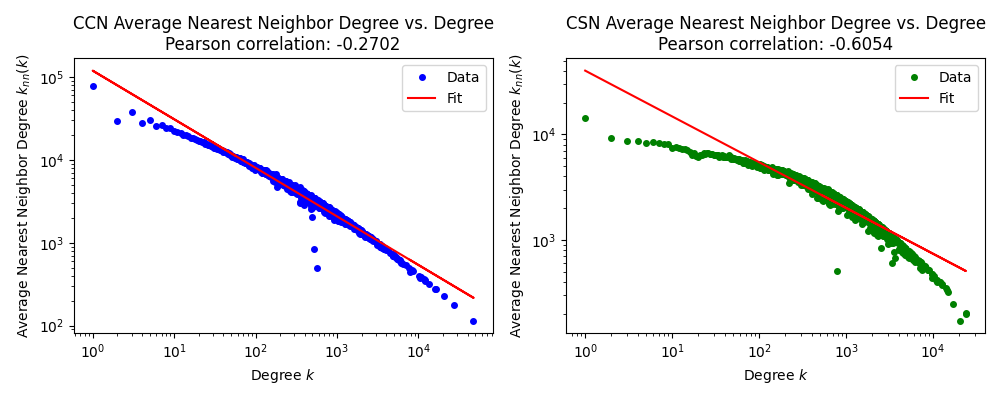
\includegraphics[width=0.8\textwidth]{../analysis/knn/knn.png}
    \caption{Degree correlations in CCN and CSN. The Pearson correlation coefficients are -0.2702 for CCN and -0.6054 for CSN.}
    \label{fig:degree_correlation}
    \end{figure}
    Based on the Pearson correlation coefficient, $r_1=-0.2702$ for CCN and $r_2=-0.6054$ for CSN. Our findings confirm the disassortative nature of CCN and CSN (Figure \ref{fig:degree_correlation}):
    \begin{equation}
    r = \frac{M^{-1}\sum_{i}j_ik_i-[M^{-1}\sum_{i}\frac{1}{2}(j_i+k_i)]^2}{M^{-1}\sum_{i}\frac{1}{2}(j_i^2+k_i^2)-[M^{-1}\sum_{i}\frac{1}{2}(j_i+k_i)]^2}
    \end{equation}
    High-degree function words typically associate with low-degree content words, a phenomenon known as disassortativity, which reflects syntactic and semantic constraints in language organization. Moreover, it may enhance the robustness of the language network against errors and attacks \cite{Newman, 2002}.
    In summary, our study shows that CCN and CSN exhibit a range of complex network characteristics, including hierarchical organization, small-world effect, scale-free structure, and disassortative mixing. These features provide a quantitative description of the Chinese language system and shed new light on its dynamics, structure, and function. 
\section{Discussion}

\section{Conclusion}

\section*{Acknowledgments}

\section*{Ethical Considerations and Broader Impacts}

\section*{References}

\appendix
\section*{Appendices}
\section*{Supplementary Materials}
\subsection*{Network Visualization}

\subsection*{Statistical Tests}


\subsection*{Code and Data Availability}


% References
% \begin{thebibliography}{9}
%   \bibitem{example}
%   Author,
%   \emph{Title}.
%   Publisher, Year.
% \end{thebibliography}
% \bibliographystyle{plain}
% \bibliography{references}  % replace with the actual filename of your .bib file, without the extension

\end{document}
